\documentclass[OPS,lsstdraft,authoryear,toc]{lsstdoc}
\input{meta}

% Package imports go here.

% Local commands go here.

%If you want glossaries
%\input{aglossary.tex}
%\makeglossaries

\title{LSSTCam Focal Plane Layout}

% This can write metadata into the PDF.
% Update keywords and author information as necessary.
\hypersetup{
    pdftitle={LSSTCam Focal Plane Layout},
    pdfauthor={First Last},
    pdfkeywords={}
}

% Optional subtitle
% \setDocSubtitle{A subtitle}

\author{%
Andrés A. Plazas Malagón, Seth Digel, Aaron Roodman, Alex Broughton, the LSST Camera Team. 
}

\setDocRef{CTN-001}
\setDocUpstreamLocation{\url{https://github.com/lsst/ctn-001}}

\date{\vcsDate}

% Optional: name of the document's curator
% \setDocCurator{The Curator of this Document}

\setDocAbstract{%
This document includes figures of the LSST Camera’s focal plane layout with ITL and e2v CCDS, highlighting the arrangement of science, wavefront, and guider sensors.
}

% Change history defined here.
% Order: oldest first.
% Fields: VERSION, DATE, DESCRIPTION, OWNER NAME.
% See LPM-51 for version number policy.
\setDocChangeRecord{%
  \addtohist{1}{2025-02-27}{Create document.}{Andrés A. Plazas Malagón, Seth Digel}
}

\begin{document}

% Create the title page.
\maketitle
% Frequently for a technote we do not want a title page  uncomment this to remove the title page and changelog.
% use \mkshorttitle to remove the extra pages

% ADD CONTENT HERE
% You can also use the \input command to include several content files.

\section{Introduction}
This document provides an overview of the LSSTCam focal plane layout.
Figures \ref{fig:focal_plane_1} and \ref{fig:focal_plane_2} below illustrate the placement of science, wavefront, and guider sensors, from both ITL and e2v.
The view is looking down from above the focal plane, i.e., through the LSSTCam lenses.

Figure \ref{fig:focal_plane_2} also includes the serial numbers of the raft tower modules (RTM-\#\#\#), the corner raft tower modules (CRTM-\#\#\#), and the individual CCDs.
The latter are the three-digit numbers immediately below the positional designator of the CCD.
For example, R11\_S10 is E2V-CCD-354) and R20\_S10 is ITL-CCD-351.
The raft and CCD serial numbers come from the \emph{eTraveler} database accessed using {\tt{datacat-utilities}}\footnote{\url{https://github.com/lsst-camera-dh/datacat-utilities}}.

The set of dead segments and high-noise segments is somewhat dynamic; dead or high-noise segments sometimes revive/recover and functioning segments sometimes die or become noisy.
The set of bad segments indicated in the figures is current as of the end of Run 7 electro-optical testing.

Figure \ref{fig:focal_plane_3} shows the LSSTCam photographed in the LSST clean room, with the camera rotated 90 deg clockwise with respect to the diagrams in Figures \ref{fig:focal_plane_1} and \ref{fig:focal_plane_2}.
For more comprehensive technical details on the layout of the CCDs in the focal plane, consult the reference document LCA-13381 \citep{lca13381}. 

The source code used to generate the figures is available in the GitHub repository associated with this Camera Technical Note.

\clearpage

\begin{figure}
  \centering
  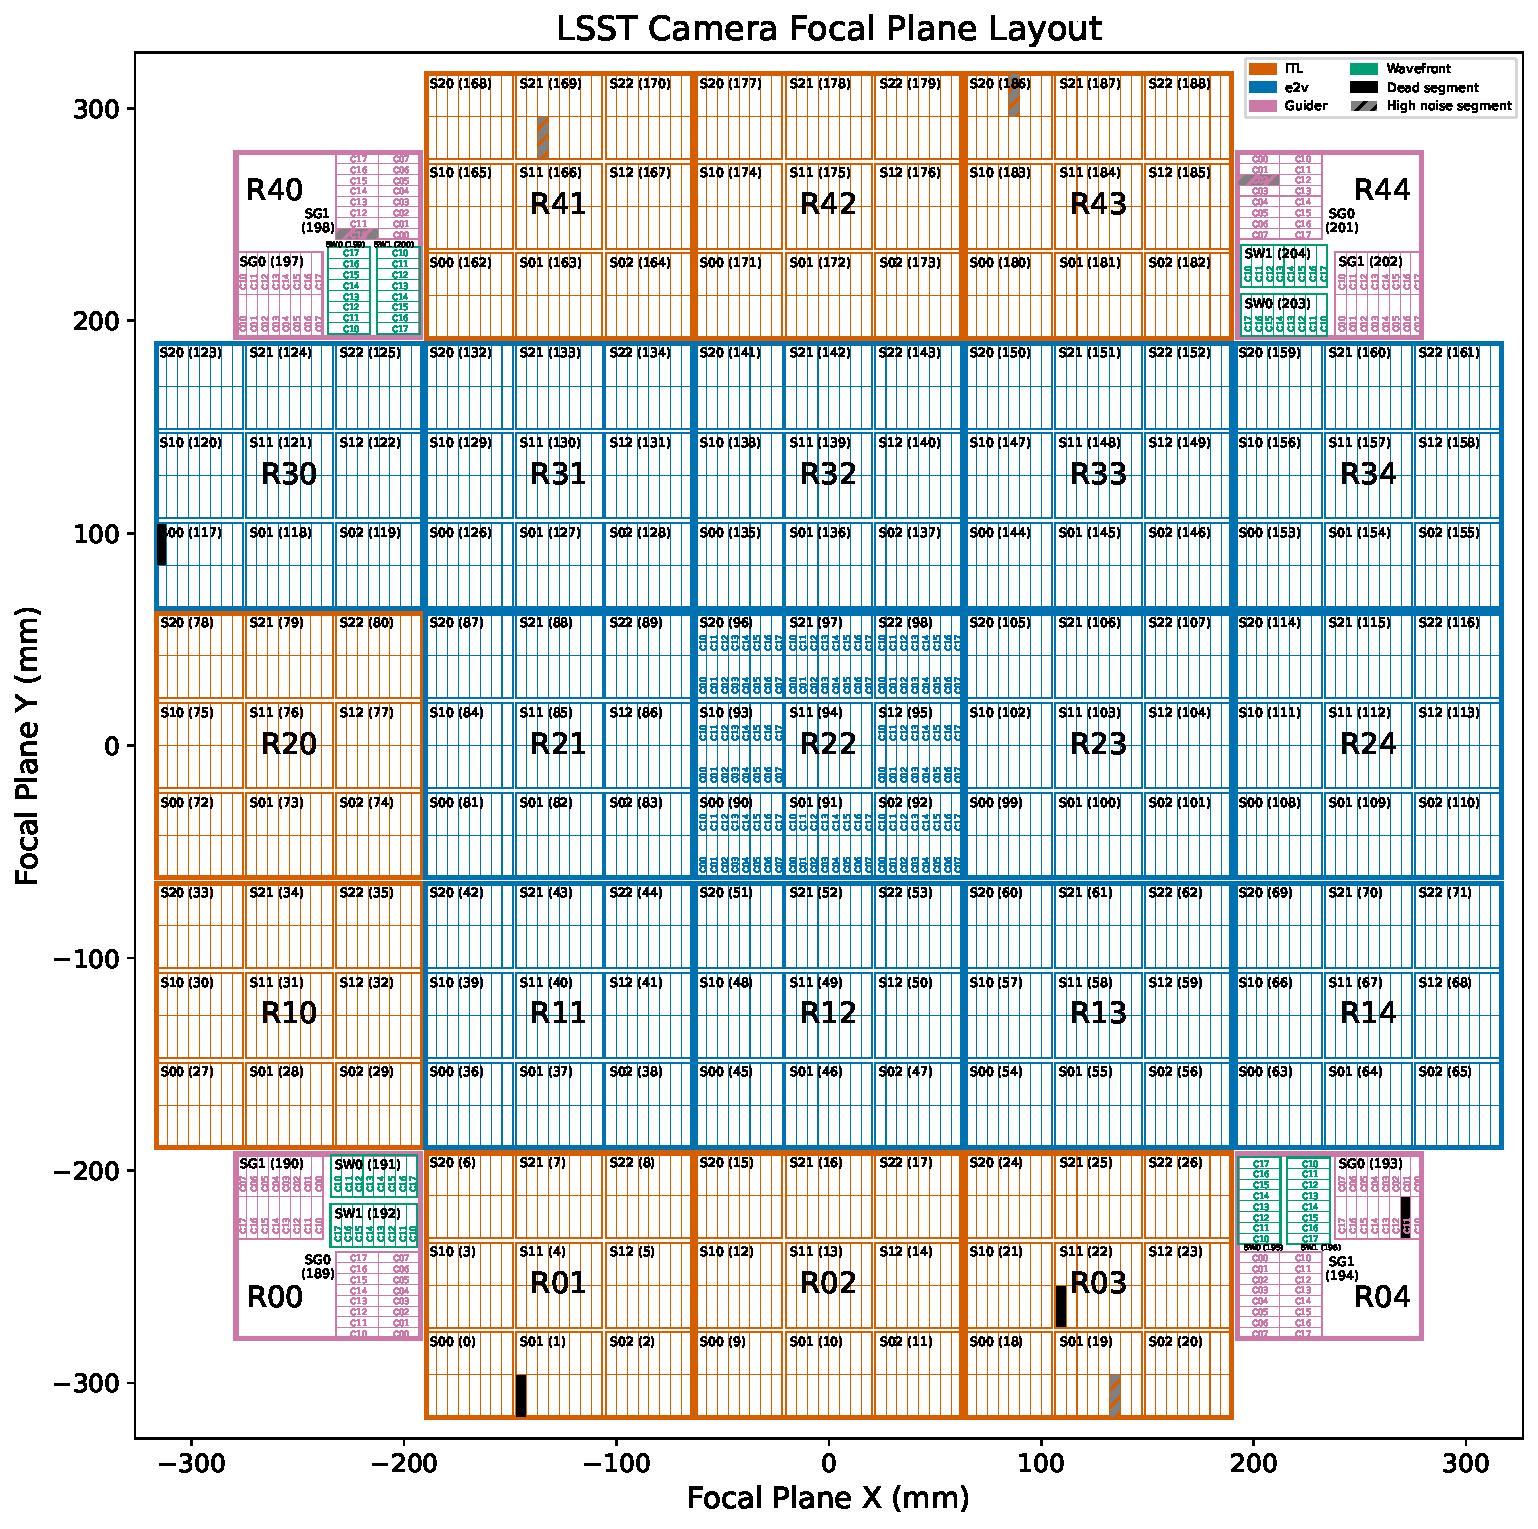
\includegraphics[width=\textwidth]{figures/LSSTCam_focal_plane_andres_2025MAR03.pdf}
  \caption{Focal plane layout. The list of ``dead'' (readout noise $> 4\,\mathrm{e}^{-}$ or anomalous Photon Transfer Curve gain) 
	amplifiers (segments) is {\tt{R30\_S00\_C10}}, {\tt{R01\_S01\_C00}}, {\tt{R03\_S11\_C00}}, {\tt{R04\_SG0\_C11}} 
and the list of ``high-noise'' (readout noise $> 18\,\mathrm{e}^{-}$) amplifiers is 
{{\tt{R41\_S21\_C02}}, {\tt{R43\_S20\_C14}}, {\tt{R03\_S01\_C05}}, {\tt{R40\_SG1\_C10}}, 
	{\tt{R44\_SG0\_C02}}, taken from Tables~8 and 9 of SITCOMTN-148 \citep{utsumi25}. Code source: \url{https://github.com/lsst/ctn-001/code/}}}
  \label{fig:focal_plane_1}
\end{figure}

\clearpage

\begin{figure}
  \centering
  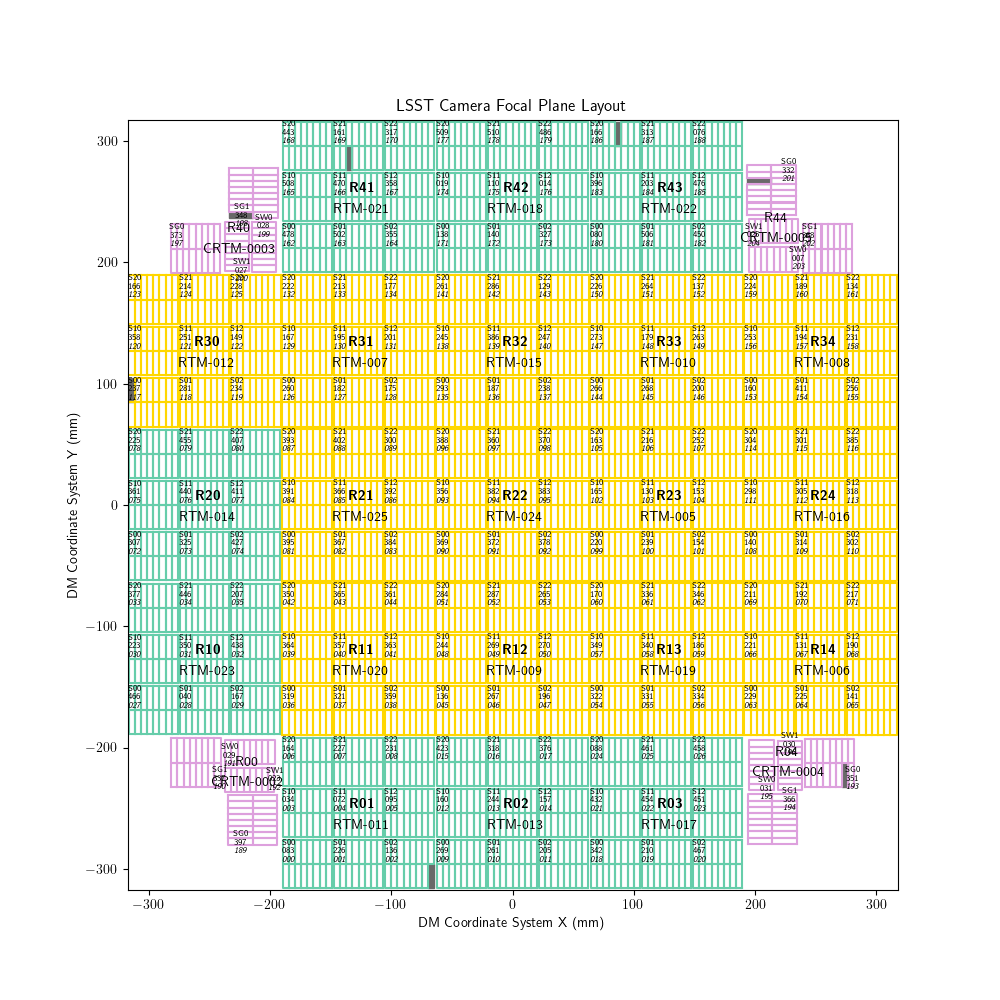
\includegraphics[width=\textwidth]{figures/LSSTCam_fp_layout_seth_Oct2024.png}
  \caption{Focal plane layout including raft and CCD serial numbers (see text). The raft and CCD serial numbers come from the \emph{eTraveler} database accessed using {\tt{datacat-utilities}} (\url{https://github.com/lsst-camera-dh/datacat-utilities}). The bad segment list is current as of October 7, 2024.}
  \label{fig:focal_plane_2}
\end{figure}

\clearpage

\begin{figure}
  \centering
  \includegraphics[width=\textwidth]{figures/LSSTCam_photo.jpg}
  \caption{LSSTCam photographed in the LSST clean room on January 16, 2024. (Jacqueline Ramseyer Orrell/SLAC National Accelerator Laboratory). The camera is rotated 90 deg counter-clockwise with respect to the diagrams in Figures \ref{fig:focal_plane_1} and \ref{fig:focal_plane_2}. Source: \url{https://rubinobservatory.org/gallery/}}
  \label{fig:focal_plane_3}
\end{figure}

\appendix
% Include all the relevant bib files.
% https://lsst-texmf.lsst.io/lsstdoc.html#bibliographies
\section{References} \label{sec:bib}
\renewcommand{\refname}{} % Suppress default Bibliography section
\bibliography{local,lsst,lsst-dm,refs_ads,refs,books}

% Make sure lsst-texmf/bin/generateAcronyms.py is in your path
\section{Acronyms} \label{sec:acronyms}
\addtocounter{table}{-1}
\begin{longtable}{p{0.145\textwidth}p{0.8\textwidth}}\hline
\textbf{Acronym} & \textbf{Description}  \\\hline

CCD & Charge-Coupled Device \\\hline
ITL & Imaging Technology Laboratory (UA) \\\hline
LCA & Document handle LSST camera subsystem controlled documents \\\hline
LSST & Legacy Survey of Space and Time (formerly Large Synoptic Survey Telescope) \\\hline
OPS & Operations \\\hline
RTM & Raft Tower Module \\\hline
SLAC & SLAC National Accelerator Laboratory \\\hline
\end{longtable}

% If you want glossary uncomment below -- comment out the two lines above
%\printglossaries





\end{document}
